\documentclass[a4paper,12pt]{report}
%%%%%%%%%%%%%%%%%%%%%%%%%%%%%%%%%%%%%%%%%%%%%%%%%%%%%%%%%%%%%%%%%%%%%%%%%
%%%%%% Definizioni:
\def\titolotesi{Soluzione di problemi di direction finding con l'utilizzo di un algoritmo di posizionamento ad ancora singola} % INSERIRE TIOLO DELLA TESI
\def\laureando{Federico Dolce}       % INSERTIRE NOME COGNOME LAUREANDO
\def\annoaccademico{2012-2013}    % INSERIRE ANNO ACCADEMICO
\def\dedica{Alla mia famiglia}      % INSERIRE DEDICA
%%%%%% File previsti in input:
%% introduzione.tex    (deve contenere solo il testo, senza \chapter{})
%% capitolo1.tex       (deve iniziare con \chapter{titolo capitolo})
%% capitolo2.tex                           "
%% capitolo3.tex                           "
%% capitolo4.tex                           "
%% conclusioni.tex     (deve contenere solo il testo, senza \chapter{})
%% appendice.tex       (deve contenere solo il testo, senza \chapter{})
%%%%%%%%%%%%%%%%%%%%%%%%%%%%%%%%%%%%%%%%%%%%%%%%%%%%%%%%%%%%%%%%%%%%%%%%%

% Title Page
\title{\begin{large}\textbf{\titolotesi}\end{large}}
\author{\laureando}
\usepackage[utf8]{inputenc}
\usepackage[italian]{babel}
\usepackage{fancyhdr}
\usepackage[hidelinks]{hyperref}
\fancyhf{}
%\fancyhead[RO]{\the\chaptermark}
%\[LE,RO]{\bfseries\thepage \hfil}
\usepackage{epsfig}
\pagenumbering{roman}
%\usepackage{setspace}
\newlength\sinistra
\newlength\corpo
\newlength\pagina
\setlength {\pagina} {21cm}
\setlength {\sinistra} {1.46cm}
\setlength {\corpo} {13.5cm}
\textwidth \the\corpo
\hoffset \the\sinistra
\paperwidth \the\pagina
\linespread{1.6}


\begin{document}
\begin{titlepage}
%\maketitle
 \begin{center}
\textsc{\Large Universit\`a degli Studi di Perugia}\medskip\\

{\Large Facolt\`a di Scienze Matematiche, Fisiche e Naturali}\medskip\\

\rule{10mm}{0.01mm}\medskip\\

{\small \textsc{Corso di Laurea in Informatica}}\medskip\\

%\vspace*{12mm}

\vspace*{3mm}


\includegraphics[scale=0.35]{logounipg.png}

\vspace*{-2.5cm}

\Large Tesi di Laurea \par\bigskip

%\vfill

%\vspace*{0.3cm}

{\large \bf \titolotesi \par}

\bigskip\bigskip

\end{center}\par
%\vspace*{0.5cm}\large

\hspace{0.05cm}Laureando:\hspace{7.3cm}Relatori:\par

\hspace{0.0cm}\emph{\laureando}\hfill\emph{Prof.~Osvaldo Gervasi, Dott. Emanuele Palazzetti}

\begin{center}

\rule{40mm}{0.01mm}\\

Anno Accademico \annoaccademico

\end{center}

\end{titlepage}
\newpage
\vspace*{2.5cm}
\begin{flushright}
\begin{Large}\emph{\dedica}\end{Large}
\end{flushright}
\frenchspacing
%%%%%% Ringraziamenti (opzionale)
%
%\chapter*{Ringraziamenti}
%Voglio ringraziare ....
%%%%%%%%%%%%%%%%%%%%%%%%%%%%%%%%%
\tableofcontents
\listoffigures
\pagenumbering{arabic}
%%%% fine prologo
%%%% Inizio corpo tesi
\pagestyle{fancy}
\fancyhead[RO]{\bfseries Introduzione}
\fancyfoot[LE,RO]{\thepage \hfil}
\addcontentsline{toc}{chapter}{Introduzione}
\chapter*{Introduzione}
Lo sviluppo e la costante diffusione di tecnologie di comunicazione wireless aprono nuove frontiere per la progettazione e la realizzazione di dispositivi connessi fra di loro. Basti pensare ai sistemi di geolocalizzazione presenti negli smartphone che permettono di avere informazioni riferite al luogo in cui ci si trova in tempo reale, o ai navigatori gps, già in largo uso da diversi anni. Questa evoluzione è andata di pari passo con nuove tecniche di "context awereness" che hanno permesso ai dispositivi di riconoscere il tipo di ambiente in cui si trovano, attraverso l'analisi di dati provenienti da sensori così da reagire di conseguenza. 

Ad esempio uno smartphone "cosciente" del contesto in cui si trova, potrebbe riconoscere una stanza dove è in corso una riunione e rifiutare una chiamata in arrivo. Questa funzionalità può essere estesa anche in ambito medico, dove un dispositivo può visualizzare a schermo i dati del paziente, oppure presentare i compiti da svolgere in una determinata zona dell'ospedale così da permettere di inserire o aggiornare questi dati. 

Un altro possibile scenario, visto il crescente interessi nei confronti di questi mezzi, riguarda i droni\footnote{aeromobile multirotore in grado di muoversi autonomamente, senza bisogno di controlli dall'esterno}. Ad esempio questi possono essere utilizzati per raggiungere parti del mondo in cui le strade non sono utilizzabili se non in brevi periodi dell'anno, per portare cibo medicinali e beni di prima necessità. Come propone Andreas Raptopoulos durante la conferenza TED Global di giugno 2013
\footnote{ \url{http://www.ted.com/talks/andreas_raptopoulos_no_roads_there_s_a_drone_for_that} }, sviluppare un network di basi di atterraggio e ricarica per droni che copra una vasta superficie geografica è molto più economico, veloce, ed ecocompatibile della costruzione e manutenzione di arterie stradali o ferroviarie.

Nel nostro lavoro di tesi si è riprodotto proprio quest'ultimo problema, attraverso un software che simula questa situazione. È stato scelto di utilizzare il linguaggio di programmazione Python, già utilizzato in altri progetti che sviluppano tecniche di context-awareness.

È stato creato un sistema di gioco all'interno del quale fosse possibile sviluppare l'algoritmo di controllo del drone che permettesse di calcolare il percorso da fare per raggiungere un punto nello spazio. Per analizzarne il comportamento è stato sviluppato un software di benchmark che permettesse di valutarne la bontà in maniera sistematica, simulando quante più configurazioni possibili.

Durante tutto questo processo è stato svolto un lavoro di ricerca che ha permesso di inquadrare la tipologia del problema.

Nel primo capitolo sarà introdotto il concetto di direction finding e saranno spiegate le diverse tecniche impiegate per risolvere il problema. 

Nel secondo capitolo si affronta il problema dal punto di vista del "positioning", ovvero della localizzazione di un punto in uno spazio geografico. 

Nel terzo capitolo viene analizzato tutto il lavoro svolto nella fase di implementazione, evidenziandone le parti più importanti, entrando anche nel dettaglio delle varie componenti create.

Il quarto capitolo contiene i risultati della suite di benchmark, e le conseguenti riflessioni.        %Il testo delkl'introduzione e' in un file esterno: "introduzione.tex"

%%%%%%%%%%%%%%%%%%%%%%%%%%%%%%%%%%%%%%%%%%%%%%%%%%%%%%%%%%%%%%%%%%%%%%%%%%%%%%%%%%%%%
% Capitolo 1
%\chapter{Titolo capitolo primo}                 %%% OGNI CAPITOLO INIZIERA' CON QUESTE DUE ISTRUZIONI!
%\fancyhead[RO]{\bfseries Titolo capitolo primo} %%%

\chapter{Problemi di direction-finding}
\fancyhead[RO]{\bfseries Problemi di direction-finding}
\section{Introduzione dei problemi di direction finding}

L'obiettivo delle tecniche di direction finding (DF) è quelllo di determinare la direzione di provenienza di un segnale trasmesso da un'emittente radio, misurando e valutando alcuni parametri dei campi elettromagnetici. Per determinare la direzione è in generale sufficiente calcolare l'azimut\footnote{L'azimut è la distanza angolare compresa tra la direzione del Nord e la direzione in cui cade la perpendicolare di un punto all'orizzonte, calcolata muovendosi in senso orario.}. A questa, solitamente, va sommato il calcolo dell'altitudine, qualora il DF venga installato su una piattaforma volante. Solo nel caso di una propagazione delle onde priva di disturbi la direzione del segnale emesso coincide con quella del segnale ricevuto. L'apparecchio che esegue il direction finding, prende in considerazione le onde ricevute, e le analizza cercando di approsimare al meglio la direzione di arrivo del segnale.

In questo capitolo vengono introdotte le tecniche utilizzate in diversi campi per risolvere questo tipo di problea. In particolare viene spiegato il sistema basato sulla potenza del segnale ricevuto, che è il metodo utilizzato per questo lavoro. 

\subsection{Utilizzi delle tecniche di direction finding}
Sebbene le tecniche di DF legate alla navigazione non siano molto diffuse, data la presenza dei sistemi di navigazione satellitare, la loro richiesta aumenta nei campi dove è importante determinare la posizione di antenne riceventi e trasmittenti. Alcuni casi d'uso riguardano i servizi di sicurezza in cui è richiesto di rintracciare l'origine di comunicazioni radio emesse da organizazioni criminali; l'intelligence militare, per rivelare possibili attività nemiche, o svelare posizioni o ordini impartiti via radio; in ambiti di ricerca quali la radio astronomia o il sensing remoto di dati raccolti. 

Un altro fattore che rende importanti queste tecniche, è il costante aumento delle comunicazioni wireless. Il direction finding è quindi un primo passo fondamentale per la localizzazione radio, specialmente quando il contenuto di queste trasmissioni non può essere letto. La localizzazione delle emittenti è di solito un processo suddiviso in diverse fasi: 
\begin{itemize}
\item Emittenti posizionate in un largo spazio geografico che possono approsimare la posizione con una precisione di pochi chilometri attraverso la triangolazione radio;
\item La posizione dell'emittente può essere raffinata utilizzando riceventi collocate nei veicoli; 
\item Sistemi di DF portatili che permettono di ridurre la ricerca nel raggio di un centinaio di metri, ad esempio all'interno di un edificio.
\end{itemize}


\subsection{Classificazione dei sistemi di direction finding}

In letteratura è presente un vasto assortimento di algoritmi e sistemi per la soluzione di problemi di DF.
I sistemi di "radio direction finding" utilizzano una seria di antenne e una o più riceventi o per stimare un angolo di rilevamento o per determinare le coordinate geografiche di un segnale ricevuto (SOI\footnote{SOI: Signal Of Interest}). La funzione primaria di un sistema di DF è quella di calcolare la direzione di arrivo (DOA\footnote{DOA: Direction Of Arrival}). 
Gli algoritmi di DF sono di solito divisi in due categorie: sistemi di DF ad n canali, che utilizzano un canale della ricevente per ogni antenna; sistemi di DF a canale singolo, che utilizzano una singola antenna, una serie di trasmettitrici e un sistema che permetta di passare da un segnale all'altro, o che combini i segnali in modo da poterli presentare alla ricevente come un segnale singolo. I sistemi a canale singolo hanno alcuni vantaggi rispetto a quelli ad n canali, tra cui la portabilità, a discapito della potenza di calcolo o della robustezza in condizioni avverse. La sfida rappresentata dallo sviluppo di tecniche di DF a canale singolo e ciò che ne fa un interessante campo di studi è quello di ricercare un sistema che permetta di offrire prestazioni tipiche dei più complessi sistemi ad n canali, contribuendo anche allo sviluppo di questi ultimi.

Altre forme di classificazione degli algoritmi di DF prendono come parametro il modo in cui il segnale viene trattato. Gli approcci possono essere, dunque, basati sull'ampiezza del segnale (RSS\footnote{RSS: Received Signal Strenght}), sulla fase	dell'onda ricevuta, o una combinazione delle due. I sistemi basati su RSS comparano l'ampiezza ricevuta dai vari elementi nella serie di antenne per localizzare un punto nel piano vicino alle antenne dalle quali ha origine il segnale. I sistemi basati sulla fase del segnale determinano le informazioni necessarie a stabilire la DOA dalla fase assoluta, o dalla differenza di fase, dei segnali ricevuti dalle antenne. I sistemi che utilizzano entrambi i sistemi sono più complessi, ma in generale hanno prestazioni migliori.

\subsubsection{Sistemi a Tempo Di Arrivo (TOA)}

Il tempo di arrivo di un segnale che viagga da un nodo all'altro può essere utilizzato per stimare la distanza fra i due nodi. Se i due nodi sono sincronizzati, la ricevente può determinare il ToA del segnale. La sincronizzazione fra i due nodi è un punto fondamentale in questo tipo di tecnica e da questa, in genere, dipendono le prestazioni del sistema nel complesso. Per effettuare la stima della posizione sono necessari almeno 3 nodi.

\subsubsection{Sistemi a Direzione di Arrivo (DOA)}

I sistemi basati sulla direzione di arrivo utilizzano di solito stazioni ad antenna multipla. Questi sistemi sono interessanti in quanto, a differenza di altri, non hanno bisogno di una sincronizzazione fra le stazioni, e sono sufficienti due stazioni base per permettere	di effettuare la localizzazione. Ci sono molte soluzioni basate su questo approccio sviluppate negli ultimi quranta anni. Il MUSIC\footnote{Acronimo di MUltiple SIgnal Classification, si tratta di una tecnica per la stima di frequenza e per la localizzazione della direzione di provenienza di un segnale (DOA).}, l'ESPIRT\footnote{Acronimo per Estimation of Signal Parameters via Rotational Invariant Techniques (ESPRIT) è una tecnica per determinare dei parametri di un insieme di sinusoidi immerse in del rumore di fondo.} e le rispettive varianti, sono le più utilizzate in tempi recenti. Questi, pur essendo subottimali, forniscono delle ottime prestazioni e sono di solito considerati algoritmi di riferimento in questo ambito.

\subsubsection{Sistemi Received Signal Strenght (RSS)}
Queste tecniche si basano sull'idea che la potenza del segnale varia con la distanza. In questo modo la RSS inviata alla ricevente dà informazioni riguardo la distanza di questa dalla sorgente. In ogni caso è necessario stabilire una scala che permetta di convertire la differenza di potenza del segnale ricevuto (PL\footnote{PL: Path Loss}) in una distanza. Un modello comune per la PL chiamato "log-normal shadowing PL model" è dato da:
 $$ PL\left(d\right) = PL\left(d_0\right) + 10n_plog_{10} \left( \frac{d}{d_0} \right) + v $$
dove:
\begin{itemize}
\item $ PL(d) $ è il PL in dB alla distanza d; 
\item $ PL(d_0) $ è il PL in dB ad una distanza relativamente breve $ d_0 < d $ ($ d_{0} $ di solito è un metro); 
\item $n_p$ è quello che è chiamato "path loss exponent". I valori di $n_p$ più comunemente utilizzati possono andare da 2 in campo aperto, o 4-6 in caso di utilizzo in un percorso ostruito da muri.
\item $v$ è una variabile gaussiana casuale che rappresenta l'effetto del "log normal shadowing". Solitamente questa variabile $v$ è considerata zero. 
\end{itemize}
Questo modello può essere utilizzato sia per utilizzi interni che all'aria aperta. 


\chapter{Soluzione del problema con un algoritmo di posizionamento ad ancora singola}
\fancyhead[RO]{\bfseries Soluzione con un algoritmo di posizionamento ad ancora singola}
\section{Problemi di posizionamento}
Il problema del posizionamento consiste nello stabilire il punto geografico in cui si trova un oggetto. In ambienti aperti, e per le lunghe distanze, vengono spesso utilizzati sistemi GPS, la cui evoluzione ha reso possibile la loro integrazione negli smartphone e nei dispositivi embedded a costi contenuti. Questa tecnologia ha dei limiti in quanto, ad esempio, non funziona all'interno di edifici e perde di precisione in condizioni atmosferiche avverse. Per questo, problemi di posizionamento a medio-corto raggio, richiedono tutt'ora l'impiego di tecnologie  e metodi differenti. 

Un possibile approccio prevede l'utilizzo di ""ancore''. Un'ancora è un dispositivo in gradi di raccogliere dati attraverso dei sensori e di trasmetterli ad una ricevente. La ricevente memorizza i dati raccolti dalle ancore ed effettua i calcoli necessari. La comunicazione tra le ancore e la ricevente può essere implementata tramite onde radio. Si cerca quindi di stabilire la posizione relativa di una serie di ancore, rispetto ad una ricevente che si trova nall'interno dello spazio coperto dal segnale delle stesse.

A questo fine sono utilizzati algoritmi e sistemi basati su reti di sensori che comunicano o con un nodo centrale o tra di loro, scambiandosi informazioni riguardo l'ambiente in cui si trovano. Grazie a questi è possibile stabilire la posizione di ogni ancora rispetto alle altre e raccogliere dati su un ambiente al fine di descriverlo. 

Questi sono sistemi di ""radio positioning'' che utilizzano le tecniche precedentemente descritte, quali il DF basato sul tempo di arrivo del segnale, la misurazione di fase o la misurazione RSS. Ognuna di queste tecniche può essere usata a tale scopo e la differenza sta nel tipo di tecnologie utilizzate, nel costo dell'attrezzatura necessaria, nella richiesta energetica e nell'accuratezza del risultato finale.
In generale sono previsti almeno quattro nodi in uno spazio tridimensionale, così da avere una buona accuratezza nel rilevamento di un punto in uno spazio non noto. 

In questo lavoro sarà introdotto un algoritmo geometrico che permette questo tipo di localizzazione in una simulazione a due dimensioni, con una sola ancora e una ricevente mobile. L'utilizzo di una sola ancora comporta dei vantaggi dal punto di vista di costo ed energia richiesta. Si riduce quindi il numero di componenti necessari, utilizzando tecnologie presenti in ogni dispositivo in grado di comunicare via radio ed utilizzando quindi un algoritmo con un'impronta in memoria relativamente ridotta.
	
\section{Risoluzione di problemi di direction finding con il metodo di posizionamento ad ancora singola}
L'idea è quella di determinare la posizione di una singola ancora sorgente attraverso una ricevente mobile, che effettui misurazioni ad ogni passo percorso nello spazio. La tecnica utilizzata sarà la misurazione della potenza di segnale (RSS). Questa verrà convertita in distanza utilizzando una scala di conversione come quella presentata nel primo capitolo.

La principale differenza con gli approcci comunemente usati sta nell'utilizzo di una singola ancora. 
Il vantaggio di questo approccio è il basso costo dei componenti, in quanto è necessaria una singola ricevente ed un singolo trasmettitore, piuttosto che sensori o costosi apprecchi in grado di rilevare il tempo di ricezione con un errore di pochi microsecondi.

Per trovare un algoritmo di risoluzione del problema descritto si è scelto di operare all'interno di una simulazione ideale del mondo, in cui si trascurano gli errori di rilevazione, la presenza di interferenze del segnale, problematiche strettamente correlate alla meccanica di spostamento ed a tutte le problematiche che sarebbero affrontate in fase d'implementazione reale. Per stabilire la bontà dell'algoritmo stesso è stato preso come indice il numero di spostamenti effettuati dall'agente prima di raggiungere la posizione della sorgente.

Il problema da affrontare è quindi la scelta della direzione in cui far muovere la ricevente, per permettere di raggiungere la posizione della sorgente nel minor numero di passi possibile. Il problema sarà risolto utilizzando un approccio geometrico. Il mondo sarà rappresentato come una matrice in cui la ricevente potrà muoversi di un passo alla volta. La rilevazione della potenza del segnale diviene quindi il valore di ogni elemento, che non varierà durante l'esecuzione dell'algoritmo poichè la sorgente resterà fissa in un punto dello spazio. Tale valore rappresenta la distanza euclidea tra l'elemento della matrice ed il punto in cui si trova la sorgente. La ricevente potrà muoversi in ognuna degli elementi adiacenti nella matrice, consentendo anche spostamenti in diagonale. 

Poiché la simulazione è stata sviluppata in maniera modulare, è possibile confrontare l'algoritmo sviluppato con altri algoritmi. È anche possibile utilizzare l'algoritmo stesso in ambiti diversi, purchè venga mantenuta la stessa interfaccia di programmazione. Inoltre, la suite di test fornisce dati statistici utili a valutare la bontà di un qualsiasi algoritmo sviluppato per risolvere lo stesso tipo di problema. 

\chapter{Implementazione agente di ricerca}
\fancyhead[RO]{\bfseries Implementazione agente di ricerca}
La situazione inizialmente posta è stata quella di permettere ad un mezzo autonomo (ovvero in grado di operare senza azione esterna) come un robot dotato di ruote o un multirotore, di raggiungere una postazione in grado di emettere un segnale. È stato quindi sviluppato un algoritmo in grado di eseguire i passi necessari all'interno di una simulazione astratta del mondo. Il problema è quindi quello tipico del radio direction finding. Verrà qui introdotto il concetto di "ricerca", necessario per definire più formalmente il problema. In seguito viene presentata l'implementazione software del problema, descrivendo prima la suddivisione logica del software, spiegandone l'utilizzo, e infine analizzando più nel dettaglio i singoli moduli che ne fanno parte, evidenziando le parti di codice più rilevanti.

\section{Ricerca e informazione imperfetta}
È definito "agente" una qualunque entità in grado di percepire l'ambiente circostante attraverso dei sensori, e di eseguire delle azioni attraverso degli attuatori. Nel campo dell'intelligenza artificiale è definito intelligente quell'agente che fa la cosa giusta al momento giusto. È quindi necessario stabilire anzitutto quale sia l'obiettivo. Il compito dell'agente è quello di stabilire una sequenza di azioni che portano al raggiungimento di uno stato obiettivo. 
La formulazione del problema è il processo che porta a decidere, dato un obiettivo, quali azioni e stati considerare. La considerazione degli stati è strettamente legata alle informazioni che l'agente dispone e che se non avesse non potrebbe fare altro che scegliere a caso. In generale un agente che ha a disposizione diverse opzioni immediate di valore sconosciuto, può decidere cosa fare esaminando diverse possibili sequenze di azioni che portano a stati di valore conosciuto, scegliendo quindi la sequenza migliore. Questo processo di selezione è detto ricerca, la cui implementazione ha come input un problema e restituisce la soluzione sotto forma di sequenza di azioni. La fase in cui l'agente svolge le azioni è detta esecuzione.
Fondamentale nel permettere di sviluppare una sequenza di scelte adeguate, è la fase di astrazione del problema, fatta per semplificare le condizioni in cui si è sviluppato l'algoritmo, prescindendo da problemi di carattere pratico. Un'astrazione è valida se possiamo espandere ogni soluzione astratta in una soluzione nel mondo dettagliato; l'utilità è quindi quella di rendere più facile l'esecuzione delle azioni nel mondo astratto rispetto a quello originale. 
Nel problema analizzato l'agente dispone di informazioni limitate sullo stato del mondo, in quanto quest'ultimo non è completamente conosciuto dall'agente. È stato quindi necessario sviluppare una tecnica apposita, in quanto non si sarebbe potuto utilizzare un algoritmo classico di ricerca informata, quali l'A* o algoritmi greedy, perchè questi ultimi necessitano di informazione completa sugli stati del mondo, e non sarebbe stato conveniente utilizzare un algoritmo di ricerca completamente non informata, perchè non si sarebbe sfruttata l'informazione sugli stati in cui man mano l'agente si trova.


\section{Definizione delle componenti}
L'intero sistema può essere suddiviso in entità, che caratterizzano il problema. 
Le componenti che definiscono il mondo simulato sono:
\begin{itemize}
\item \textbf{Mondo}

\item \textbf{Agente}

\item \textbf{Knowledge Base (KB)}

\item \textbf{Gioco} 	
\end{itemize}

\subsection{Mondo}
Il "mondo" è un'astrazione semplificata di un possibile campo di esecuzione, in cui si prendono in considerazione solamente gli elementi necessari all'esecuzione dell'algoritmo. Questo è rappresentato sotto forma di matrice M di dimensioni $n$x$n$. Un punto di coordinate $(x_{end}, y_{end})$ o $M[x_{end}][y_{end}]$, rappresenta lo stato-obiettivo, in cui è memorizzato un valore numerico negativo. In tutti gli altri punti viene memorizzato un valore float che indica la distanza euclidea del punto in cui il valore è memorizzato, dal punto $M[x_{end}][y_{end}]$. La formula sarà quindi:
$$\sqrt{|(x_{end} - x)^2 + (y_{end} - y)^2|}$$
Ad esempio nel punto $(x_{end}+1, y_{end})$ sarà memorizzato il valore "1.000", nel punto $(x_{end}+1, y_{end}+1)$ il valore "1.414", nel punto $(x_{end}, y_{end})$ il valore "-1". In questo modo l'agente è in grado di sapere quando l'obiettivo è stato raggiunto, in quanto l'unico valore negativo nella matrice sarà quello del punto di arrivo, mentre tutti gli altri saranno utili alla risoluzione del problema.
L'agente è libero di muoversi in ognuno dei punti di coordinate $ x, y $ tali che $ (x-1) \le x \le (x+1), (y-1) \le y \le (y+1) $.

\subsection{Agente}
L'agente è rappresentato da una classe, chiamata "Drone", che nel momento in cui viene istanziata inizializza le componenti necessarie a memorizzare le informazioni necessarie alla ricerca. All'interno si trovano diversi metodi: il metodo che permette l'effettivo spostamente sul mondo, il metodo per l'acquisizione delle misurazioni provenienti dal mondo ed anche un metodo che permette di stampare a video il mondo secondo i dati raccolti fino a quel momento. Questo è effettivamente l'elemento che esegue l'algoritmo di DF.

\subsection{Knowledge Base (KB)}
Il KB sono le informazioni che l'agente memorizza riguardo il mondo. Queste sono organizzate in una struttura a grafo, che viene riempito mano a mano che l'agente esegue i passi. Il grafo può crescere fino ad avere un numero di nodi al massimo pari al numero di passi eseguiti per raggiungere l'obiettivo. Per ottimizzare l'utilizzo di memoria, è stata aggiunta la possibilità di limitare il numero di nodi memorizzati nel grafo ad un intero N, con una perdita in termini di prestazioni variabile, ma che permette un buon compromesso, per determinati valori di N.

\subsection{Gioco}
Il gioco è la definizione della sequenza in cui svolgere le azioni per la simulazione: si inizializzano l'agente, il mondo ed il knowledge. Dopodichè, in un ciclo che finisce quando l'agente ha raggiunto l'obiettivo, o quando il valore "fuel" del Drone arriva a 0, si seleziona il Drone da un array, si chiama la funzione di probe del drone, per permettergli di misurare la propria distanza dal punto di arrivo, si assegnano a due variabili x ed y il risultato dell'esecuzione dell'algoritmo di ricerca vero e proprio, poi si chiama la funzione di movimento del drone con parametri queste due variabili. Alla fine del ciclo si aumenta il contatore dei passi svolti, si controlla se il drone è arrivato a destinazione, se non lo è il ciclo ricomincia, altrimenti viene annunciato il successo.

	
\section{Architettura software}
Il software è strutturato in maniera modulare, in modo da permettere il riutilizzo delle singole componenti in diversi ambiti, o di mentenere ed aggiornare i moduli senza influenzare il funzionamento dell'intero programma, a patto di mantere la stessa interfaccia.

\subsection{Pacchetto "Game engine"}
Nel pacchetto Game Engine sono presenti i moduli che permettono l'utilizzo del sistema di simulazione

\subsubsection{Game.py}
Il modulo Game.py è la classe di gioco. Nel momento in cui ne viene creata un'istanza, inizializza le componenti del gioco (mondo, droni, knowledge base). All'interno è presente la funzione di gioco "start-game" in cui vengono eseguiti i passi di ogni turno di gioco. 
\begin{verbatim}
def start_game(self):
  i = 0
  while(self.asset_not_found):
    drone = self.next_drone()
    drone.probe(self.world[drone.actual_position[0]][drone.actual_position[1]])
    x, y = drone.strategy()
    drone.move(x, y)
    i += 1
    if self.asset_found(x, y) or drone.fuel == 0:
      self.asset_not_found = False
  if drone.fuel == 0:
    return 0
  else:
    return i
\end{verbatim}
Questa funzione entra in un ciclo while che finisce in due casi: se il drone arriva a destinazione, o se il valore drone.fuel è uguale a 0. Questa variabile è stata introdotta per simulare un limite pratico al numero di passi che possono essere eseguiti. All'interno del ciclo si può notare che il Drone viene prelevato (attraverso una funzione presente nello stesso modulo) da un array. Questo per consentire la possibilità di sviluppare in seguito il gioco in maniera concorrente, facendo muovere più Droni nel mondo, e decretando vincitore il primo che raggiunge l'obiettivo. Questa funzionalità non era comunque richiesta ai fini della simulazione, quindi non è stata sviluppata. Subito dopo aver selezionato il Drone che deve fare la mossa, viene chiamata la funzione di rilevamento (probe) del valore della distanza, con parametri le coordinate della posizione attuale del drone, che riceverà dal mondo informazioni da aggiungere alla knowledge base. Viene quindi chiamata la "strategy" ovvero l'algoritmo che ritorna il punto verso cui muoversi sotto forma di coordinate cartesiane. Una volta stabilite le coordinate, viene richiamata la funzione di movimento vera e proprio del drone, si aumenta il contatore (che rappresenterà il numero di passi eseguiti prima di uscire dal ciclo, quindi l'indicatore della bontà dell'algoritmo). Infine si fa un controllo e se il "fuel" è terminato, o se il drone è giunto a destinazione, viene modificata la variabile di controllo del ciclo while e la funzione ritorna il risultato.

\subsubsection{Drone.py}
Il modulo Drone.py è la classe che rappresenta l'agente. Quando viene istanziata, viene creato il grafo che rappresenta il mondo visitato dal Drone stesso, utilizzando delle funzioni presenti nel pacchetto utils. Inoltre vengono memorizzati dati che potranno essere utili per la scelta del prossimo passo. 
All'interno della classe troviamo il metodo "move":
\begin{verbatim}
def move(self, x, y):
    self.fuel -= 1
    self.actual_position = (x, y)
    self.graph[x][y] += 1
    self.kb.add_node_coord((x, y))
\end{verbatim}
che svolge la funzione di diminuire di un'unita la variabile "fuel", aggiornare la posizione attuale e aggiungere il nodo della posizione al grafo del KB. 
La funzione "strategy":
\begin{verbatim}
def strategy(self):
    return search_far_calibration(self)
\end{verbatim}
serve semplicemente a richiamare l'algoritmo vero e proprio, e ritornare i valori x e y restituiti da quest'ultimo. 
La funzione "probe":
\begin{verbatim}
def probe(self, distance):
    self.distances.append(distance)
    self.kb.change_weight(self.actual_position, distance)
\end{verbatim}
salva il valore ricevuto dal "mondo" in un'array dinamico, che servirà per eseguire calcoli considerando le ultime n distanze misurate, ed aggiorna il grafo del KB. 
E' inoltre presente una funzione "print-world" che se richiamata stampa a schermo l'attuale situazione del gioco, rappresentando i punti della matrice del mondo con un intero che indica il numero di volte che l'agente è passato su ogni casella.

\subsubsection{DroneKnowledge.py}
Inoltre è presente una classe DroneKnowledge che rappresenta un Drone con l'informazione completa sullo stato del mondo, utilizzato per eseguire il task attraverso un algoritmo greedy ottimo, che è stato usato per confrontare la qualità dell'algoritmo qui sviluppato.

\subsection{Pacchetto utils}

\subsubsection{Nodes.py}
Il modulo "nodes.py" contiene la struttura dati che viene utilizzata per rappresentare il mondo visitato dal Drone sotto forma di grafo. In nodi sono definiti come segue:
\begin{verbatim} 
class Node(object):
  def __init__(self, k, weight, counter):
    self.k = k
    self.v = (weight, 1, counter)
\end{verbatim}
Ogni nodo del grafo è rappresentato da una coppia chiave valore. La chiave è la tupla "k" che rappresenta le coordinate del punto, e viene utilizzata come chiave di ricerca dei nodi. Il valore indicizzato è composto da una variabile intera "weight" dove viene immagazinata la misurazione effettuata dalla probe del drone, il numero 1 rappresenta il numero di volte in cui il drone è passato su un determinato nodo (in fase di creazione del nodo questo sarà necessariamente 1), e la variabile "counter", incrementata ad ogni operazione sul grafo, che serve ad indicare quando il Drone è passato l'ultima volta sul nodo (più alto è il valore, più di recente è stato utilizzato il nodo). 
La struttura a grafo è appunto composta di singoli nodi come sopra descritti. In fase di inizializzazione può essere impostata la variabile "graph-max-length" che permette di impostare un limite al numero massimo di nodi nel grafo, in caso di necessità di ottimizazione della memoria. L'interfaccia permette di prelevare il valore di un nodo date le coordinate, attraverso l'uso della funzione builtin "getitem" (ovvero si può accedere ai valori di un nodo con l'utilizzo della sintassi "grafo[(x, y)]" ). L'aggiunta di un nodo al grafo è gestita in modo da:
\begin{itemize}
\item Aggiungere un nuovo nodo se le coordinate non sono ancora presenti all'interno del grafo;

\item Aggiornare un nodo se viene richiesto l'inserimento di coordinate già presenti, aumentando di 1 il valore che indica il numero di volte in cui il drone è passato sul nodo stesso; aggiornare il valore counter, in modo da memorizzare il fatto che questo è stato l'ultimo nodo usato

\item Nel caso in cui sia stato impostato un limite alla lunghezza del grafo, eliminare il nodo usato meno di recente prima di aggiungerne uno nuovo
\end{itemize}
\subsubsection{Matrix-generator.py}
Nel modulo "matrix-generator.py" sono presenti vari tool che permettono la generazione del mondo sotto forma di matrice utili per il sistema di gioco. Ad esempio la funzione che imposta i valori che verranno poi ricavati dalla probe:
\begin{verbatim}
matrix = [[0 for i in range(size)] for j in range(size)]
for i in range(size):
  for j in range(size):
    matrix[i][j] = float(fpformat.fix(math.sqrt(math.fabs(pow((x_end - i), 2) + pow((y_end - j), 2))), 3))
matrix[x_end][y_end] = -1
return matrix
\end{verbatim}

\subsubsection{Direction-modifier.py}
Nel modulo "direction-modifier.py" sono presenti funzioni che servono a modificare la direzione finale scelta dall'algoritmo nel caso questa superi i limiti della matrice, o in generale a gestire le varie eccezioni causate dalla dimensione finita della rappresentazione del mondo, onde evitare loop o errori. Qui è definita anche la convenzione utilizzata in tutto il programma per rappresentare le 8 direzioni possibili:
\begin{verbatim}
directions = {
  0: (1, 0),
  1: (1, -1),
  2: (0, -1),
  3: (-1, -1),
  4: (-1, 0),
  5: (-1, 1),
  6: (0, 1),
  7: (1, 1),
}

get_directions = {
  (1, 0): 0,
  (1, -1): 1,
  (0, -1): 2,
  (-1, -1): 3,
  (-1, 0): 4,
  (-1, 1): 5,
  (0, 1): 6,
  (1, 1): 7,
}


d = {
  "E": 0,
  "NE": 1,
  "N": 2,
  "NO": 3,
  "O": 4,
  "SO": 5,
  "S": 6,
  "SE": 7,
}
\end{verbatim}

Ad ogni possibile spostamento in una delle caselle adiacenti è stato assegnato un numero. Le coordinate rappresentano di quanto si debba traslare sugli assi x e y. Ad esempio quindi la direzione 0, che corrisponde a (1, 0), causerà uno spostamento di +1 sull'asse x (ovvero un passo a destra), e ogni volta che il valore chiave aumento di 1, il vettore spostamento viene rotato di 45° in senso antiorario. Quindi la chiave di movimento 1 causerà un movimento nella casella in alto a destra ecc. Il dizionario "d" è un'ulteriore semplificazione, che permette di associare a questi numeri la direzione dello spostamento. Si accede a questi dizionari attraverso i metodi:
\begin{verbatim}
def get_direction(x_mod, y_mod):
  return get_directions[x_mod, y_mod]

def modifier(way):
  return directions.get(way)[0], directions.get(way)[1]

\end{verbatim}

\subsection{Pacchetto Algorithm}

\subsubsection{Algorithm.py}
All'interno del pacchetto "algorithm" sono presenti gli algoritmi di ricerca, che verranno spiegati nel dettaglio in seguito. Questi ricevono in input due coordinate cartesiane e restituiscono nella stessa forma il risultato.
	
\section{Definizione delle strategie}
La strategia per la scelta della direzione in cui muovere il Drone è suddivisa in due fasi. Una calibrazione iniziale, e una strategia di movimento per avvicinarsi nel minor numero di passi al punto di arrivo. Al fine di migliorare l'efficenza ed evitare di incorrere in loop durante il percorso, in qualsiasi punto dell'algoritmo di ricerca viene fatto un controllo sul nodo in cui l'agente si trova, e nel caso sia passato per più di tre volte nello stesso punto questo si sposta in una delle caselle adiacenti in cui è passato il minor numero di volte e viene riavviato il processo di calibrazione.
La fase di calibrazione serve a capire in quale parte del piano rispetto all'agente si trovi il punto di arrivo. 
La seconda fase consiste nel muoversi nella parte di piano in cui si trova la sorgente, aggiustando di volta in volta la direzione. Gli aggiustamenti sono fatti in modo da seguire il più possibile una traiettoria lineare, riconoscendo quando ci si trova sulla retta che conduce alla destinazione nel minor numero di passi possibile, cercando in ogni caso di evitare di passare più volte nello stesso punto.
	
\section{Esecuzione dell'algoritmo}
Durante la fase di calibrazione, l'agente si sposta quindi per prima cosa sul piano orizzontale (in direzione Est), e salva le due misurazioni fatte (nel punto di partenza e subito dopo il movimento). Dopodichè il drone si muove sul piano verticale (in direzione Nord): 
\begin{verbatim}
if STEP <= 2:
    direction = d["E"] if STEP == 1 else d["N"] if STEP == 2 \
    else drone.last_direction
    return void_directions(direction, drone)
\end{verbatim}
Una volta raccolte le tre misurazioni, queste vengono comparate per escludere le porzioni di piano in cui sicuramente non si trova la sorgente:
\begin{verbatim}
elif STEP == 3:
    sud_ovest, sud_est, nord_est = distances[:3]
    direction = "S" if sud_est < nord_est else "N" \
    if sud_est > nord_est else ""
    direction += "E" if sud_ovest > sud_est else "O" \
    if sud_ovest < sud_est else ""
    drone.last_direction = d[direction]
return go_far(drone)
\end{verbatim}

Una volta esclusi tre quadranti, il Drone inizia a muoversi nella direzione della bisettrice che taglia l'unica porzione di piano dove il punto di arrivo può trovarsi. Si muove poi in questa direzione fino a che questa porta in una posizione più vicina al punto di arrivo della precedente. A questo punto viene eseguita l'unica scelta casuale dell'algoritmo, ovvero essendo uguale la probabilità che il punto di arrivo sia sopra o sotto la bisettrice, l'agente si sposta in direzione verticale od orizzontale. Se con quest'ultimo spostamento si è allontanato dalla sorgente, l'agente si muove in direzione perpendicolare rispetto all'ultimo movimento, prendendo quindi la direzione giusta, altrimenti viene svolta ancora una valutazione: se la differenza fra l'ultima distanza e quella precedente è pari a 1, significa che il punto di arrivo è sulla retta in cui si è appena mosso, e il Drone continuerà in quella direzione fino al raggiungimento dell'obiettivo. Altrimenti continua in quella direzione, e tutto il processo viene iterato. Questa fase della ricerca si interrompe in due casi: 

Nel caso in cui, durante uno dei movimenti in diagonale, il Drone si stia allontando dalla sorgente. In tal caso viene rieseguita la calibrazione e il processo rinizia da capo;

Nel caso in cui il drone arrivi a destinazione.

\chapter{Conclusioni}
\fancyhead[RO]{\bfseries Conclusioni}
\section{Definizione del software di benchmark}
Per valutare la qualità dell'algoritmo si è rivelato utile sviluppare un software in grado di raccogliere informazioni sull'efficenza dell'algoritmo stesso in tutte le possibili combinazioni di punto di arrivo/punto di partenza in mondi di dimensioni fissate. In particolare sono stati osservati i casi peggiori, la media aritmetica dei casi, lo scarto quadratico medio, e i risultati ottenuti più frequentemente. Il software permette di testare qualsiasi algoritmo in grado di interfacciarsi con il sistema di gioco. Non essendo presenti in letteratura algoritmi che risolvessero lo stesso problema qui trattato, ho ritenuto opportuno fare un confronto con un algoritmo greedy ottimo, che ha però bisogno di informazione completa sugli stati di ogni cella del mondo (anche senza aver fatto il movimento). Il termine di paragone è quindi il rapporto tra i valori raccolti attraverso l'esecuzione dell'algoritmo ottimo e quelli ottenuti con l'esecuzione dell'algoritmo descritto, più questo si avvicina ad 1, più le prestazioni dell'algoritmo sviluppato si avvicinano a quelle dell'algoritmo ottimo. Chiaramente il rapporto non sarà mai pari ad 1 a causa della differenza delle informazioni riguardo il mondo che i due agenti hanno, quindi la valutazione ha un carattere simbolico utilizzata in questo modo. Può però diventare interessante nel caso in cui vengano sviluppati altri algoritmi atti a risolvere la stessa problematica, per un confronto alla pari.

\section{Parametri che influenzano la qualità del risultato}
Ci sono dei parametri che possono essere modificati influenzando i risultati. Uno di questi è il numero di volte in cui il Drone debba passare su uno stesso punto prima di decidere di cambiare strategia e riniziare con la calibrazione. Attraverso l'osservazione dei diversi casi si è notato che facilmente l'agente può trovarsi a passare due volte nello stesso punto durante la ricerca (nel caso ad esempio si stia allontando dalla sorgente durante un movimento in diagonale), ma, date dimensioni del mondo relativamente grandi, è probabile che incorrendo tre o più volte nello stesso punto si stia entrando in un loop di movimenti, specialmente nel caso in cui la dimensione del grafo che rappresenta il KB  sia controllata, e quindi il numero di nodi memorizzati minore del numero di passi effettuati.
Un altro parametro che influenza l'efficenza dell'algoritmo è il numero di passi in orrizontale e in verticale da far svolgere al Drone durante la calibrazione. Infatti svolgendo un solo passo per direzione, nel caso in cui l'obiettivo si trovi su uno degli assi che incrociano il punto di partenza, l'agente si muoverà comunque in diagonale, per correggere in seguito la direzione, mentre permettendo di fare due passi in orizzontale, due in verticale e uno verso il punto di partenza in diagonale, nel caso in cui l'obiettivo si trovi su uno degli assi che si incontrano nell'ultimo punto in cui ci si è spostati, il drone andrebbe direttamente nella direzione del punto di arrivo. Si è notato però che questo approccio non modifica significativamente i risultati nel caso di dimensioni del mondo relativamente grandi, e ne peggiora la media nel caso di piccole dimensioni, quindi è stato preferito far svolgere all'agente un solo passo per direzione.
	
\section{Risultati}
I risultati dell'algoritmo cambiano anche qui in base ad altre condizioni: ad esempio nel caso in cui uno fra il Drone e il punto di arrivo si trovi ai bordi della matrice. Questo perchè, in questi casi, il problema è stato affrontato cercando una soluzione che permettesse semplicemente di evitare eventuali errori di esecuzione, falsando in qualche modo l'esecuzione dell'algoritmo, in quanto la tecnica è pensata per lavorare in campo aperto, in assenza di ostacoli. L'algoritmo arriva comunque a una soluzione, ma ha bisogno di più passaggi perchè appunto questa è una situazione anomala. E' stato quindi deciso di valutare la bontà dell'algoritmo escludendo queste situazioni, effettuando i test per tutte le posizioni possibili escluse quelle che portano sicuramente ad una situazione di eccezione. Tale situazione potrebbe incorrere anche in altri casi, ma questo è parte del problema (se il Drone si allontana dal punto di arrivo e va verso il bordo pur non essendo questo situato in posizioni estreme) e quindi ci si è limitati ad escludere le situazioni sfavorevoli a priori causate da problematiche tecniche e non intrinseche al problema.
Queste sono le schermate per testare l'algoritmo su una matrice 20x20:
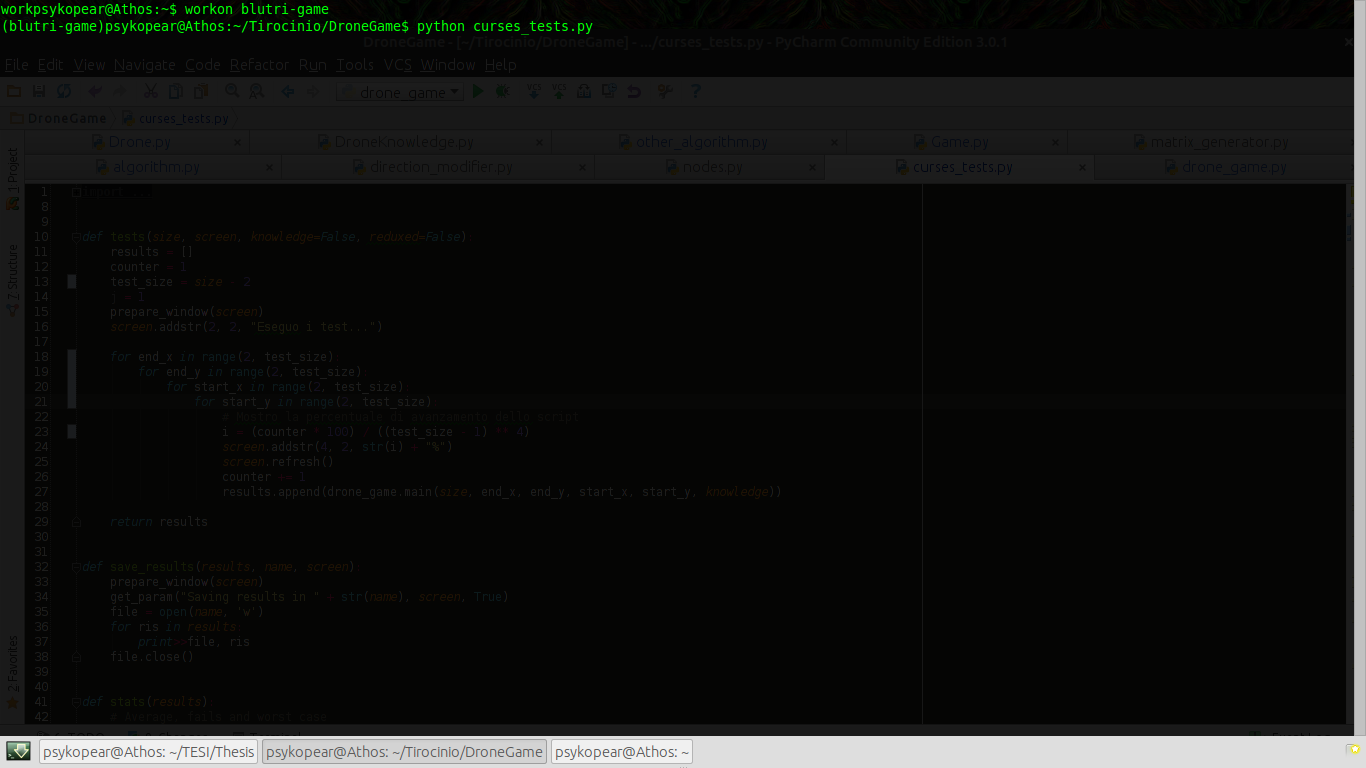
\includegraphics[width=\textwidth]{immagini/Test1.png}
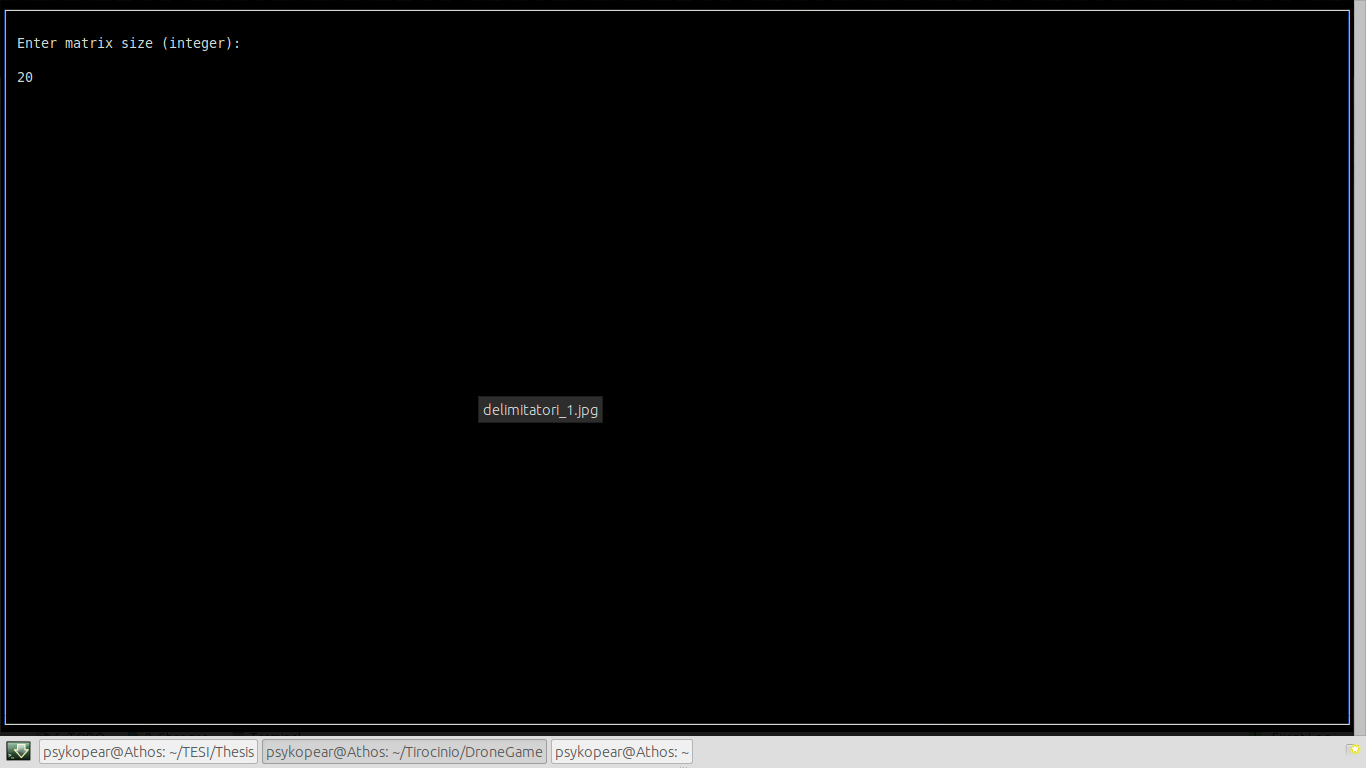
\includegraphics[width=\textwidth]{immagini/Test1-1.png}
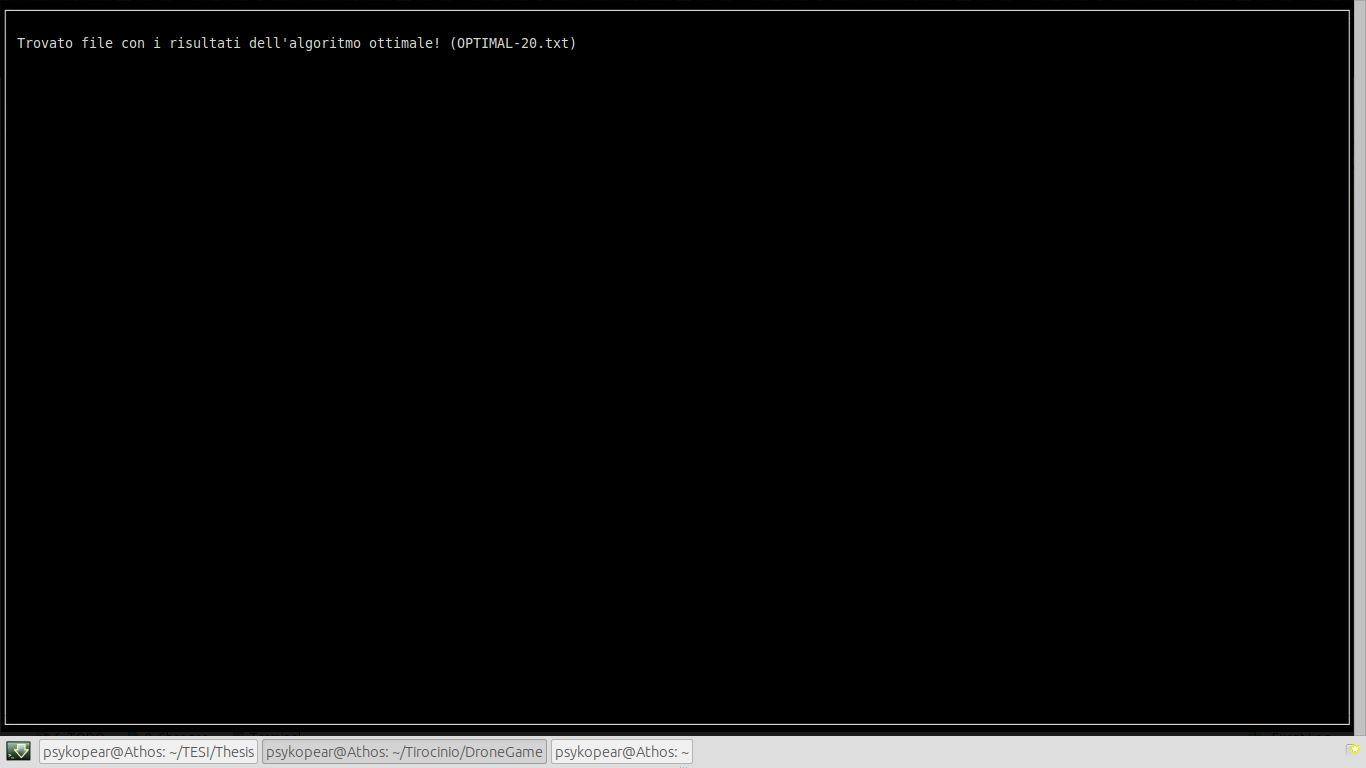
\includegraphics[width=\textwidth]{immagini/test2.png}
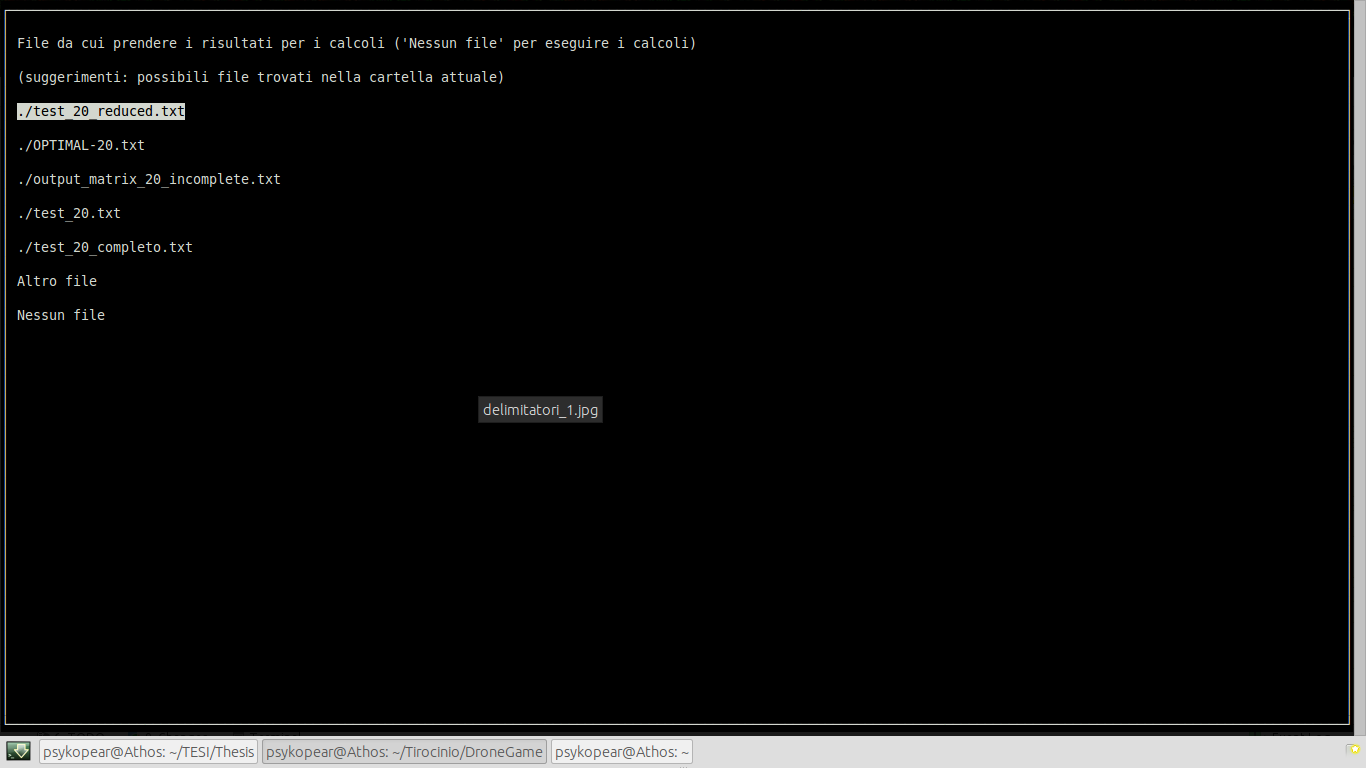
\includegraphics[width=\textwidth]{immagini/test3.png}
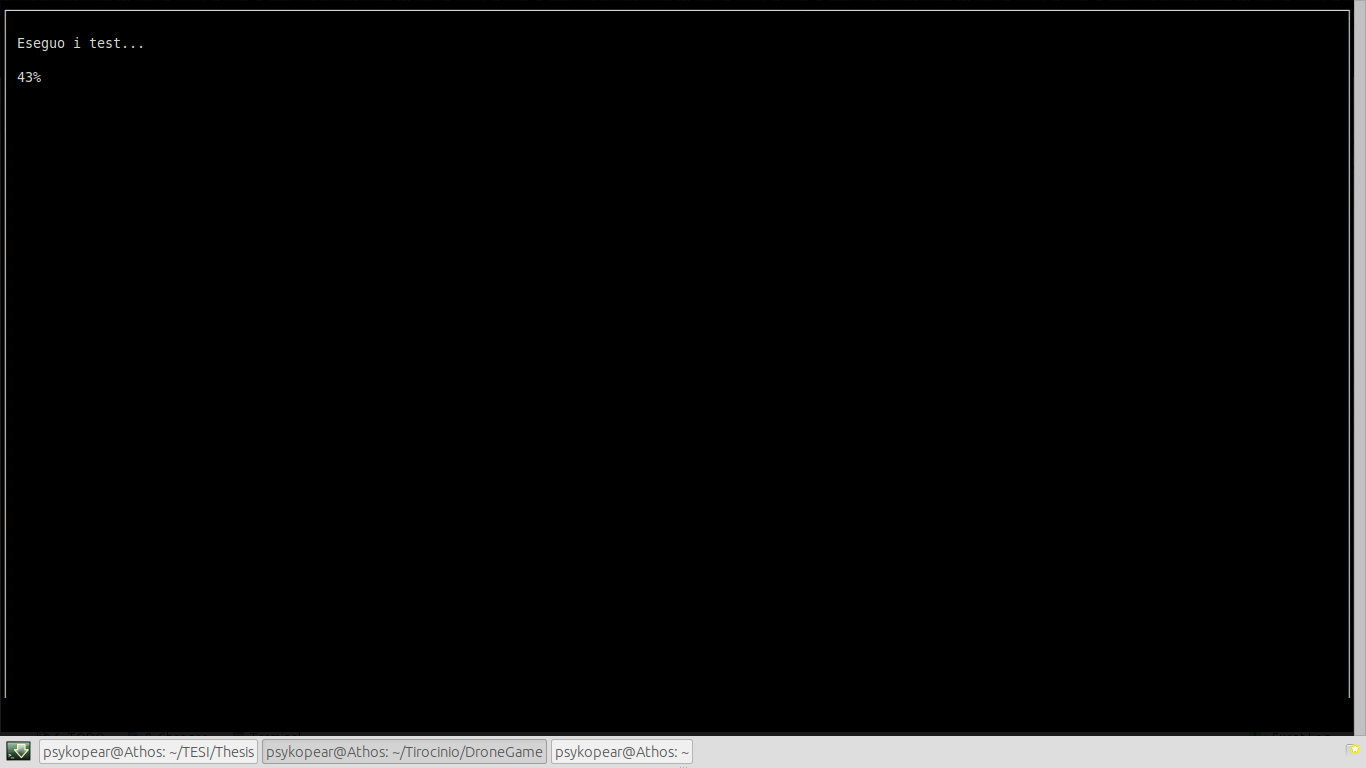
\includegraphics[width=\textwidth]{immagini/test5.png}
E questi sono i risultati ottenuti:\\*
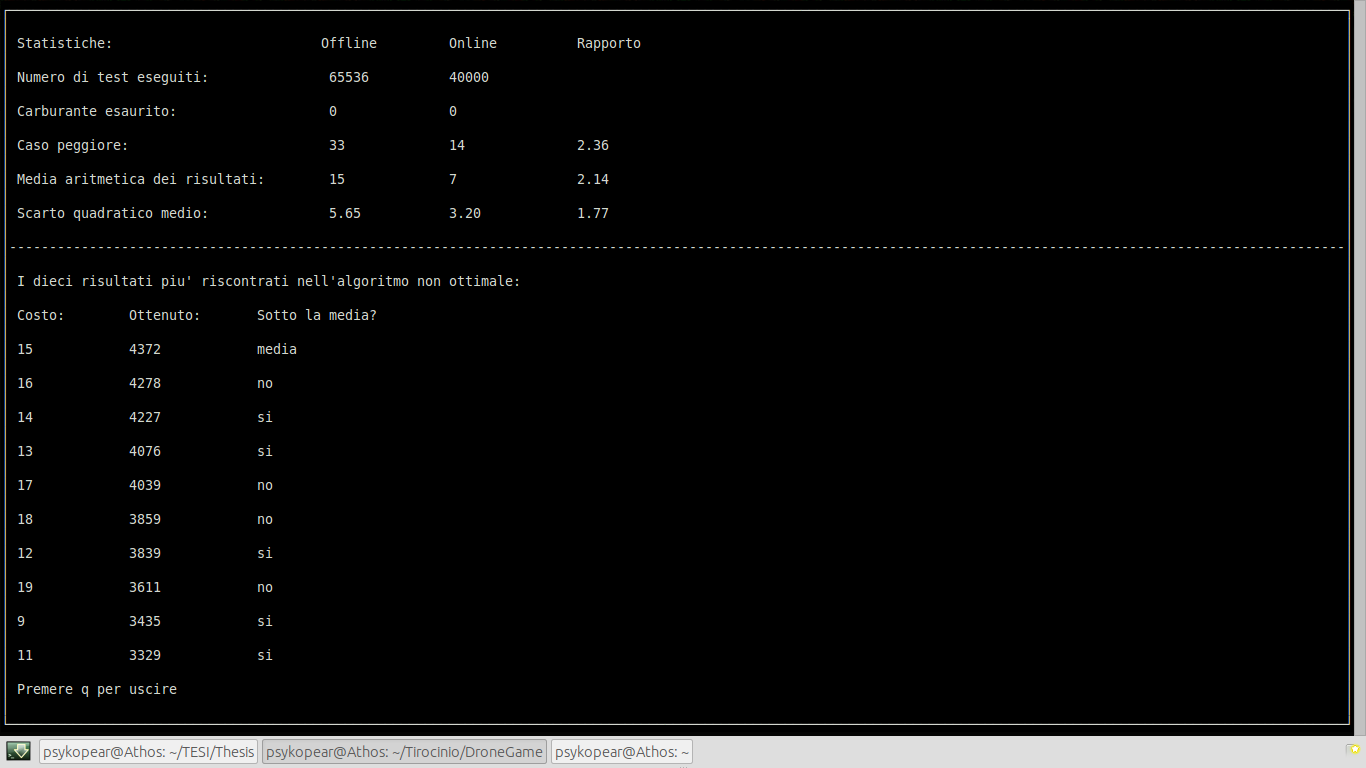
\includegraphics[width=\textwidth]{immagini/Results.png}



%%% .....
%%%%%%%%%%%% CONCLUSIONI   (non numerate come per l'introduzione)
\addcontentsline{toc}{chapter}{Conclusioni}
\fancyhead[RO]{\bfseries Conclusioni}
\chapter*{Conclusioni}

Anche la sezione Conclusioni non viene numerata...

%%%%%%%%%%%% BIBLIOGRAFIA
\newpage 
\addcontentsline{toc}{chapter}{Bibliografia}
\begin{thebibliography}{10}
\bibitem{http://static.usenix.org/event/usenix02/full_papers/savarese/savarese_html/} Robust Positioning Algorithms for Distributed Ad-Hoc Wireless Sensor Networks - 
Chris Savarese, Jan Rabaey, 
Berkeley Wireless Research Center 
\bibitem{http://scholar.lib.vt.edu/theses/available/etd-04272007-114307/unrestricted/NHarter_SingleChannelDF.pdf} Development of a Single Channel Direction Finding Algorithm - 
Nathan M. Harter
\bibitem{https://dspace-uniud.cilea.it/bitstream/10990/201/1/PhD2013_INSERRA_PDFA.pdf} Direction of arrival estimation for radio positioning:
a hardware implementation perspective - 
Daniele Inserra, Andrea M. Tonello
\bibitem{http://telekomunikacije.etf.bg.ac.rs/predmeti/ot3tm2/nastava/df.pdf} Introduction into Theory of Direction Finding - Rohde & Schwarz
\bibitem Ground-Based Wireless Positioning - Di Kegen Yu, Ian Sharp, Y Jay Guo
\end{thebibliography}
     %conterra' una serie di istruzioni del tipo:    
                         % \bibitem{eol} O. Gervasi and A. Lagan‡ "EOL: A Web-Based Distance Assessment System", 
			 % Lecture Notes in Computer Science, 3044, Springer & Verlag, pp. 854-862 (2004)

%%%% APPENDICE CON IL CODICE SVILUPPATO
\appendix
\linespread{1}
\fancyhead[RO]{\bfseries Codice}
\chapter{Allegati}
\section{Sorgente algoritmo geometrico}
Tutto il codice è disponibile su github, all'indirizzo https://github.com/Psykopear/DroneGame
\begin{verbatim}
from utils.direction_modifier import void_directions, get_direction, d
import random


def search_far_calibration(drone):

  distances = drone.distances
  STEP = len(distances)

  # Calibrazione non effettuata

  if STEP <= 2:

    direction = d["E"] if STEP == 1 else d["N"] \
    if STEP == 2 else drone.last_direction
    return void_directions(direction, drone)

  # Calibrazione effettuata, inizio a muovermi

  elif STEP == 3:

    # Le tre misurazioni della "triangolazione" per capire
    # il quadrante in cui si trova il punto d'arrivo

    sud_ovest, sud_est, nord_est = distances[:3]
    direction = "S" if sud_est < nord_est else \
    "N" if sud_est > nord_est else ""
    direction += "E" if sud_ovest > sud_est \
    else "O" if sud_ovest < sud_est else ""
    drone.last_direction = d[direction]

  return go_far(drone) 

def go_far(drone):

  if len(drone.distances) > 3 and \
  (drone.distances[-2] - drone.distances[-1]) < 0:

    if drone.last_modifier == 0:

      drone.last_modifier = 1 if random.random() < 0.5 else -1

    if not drone.flipflop:

      drone.flipflop, drone.last_direction = (True, \
      (drone.last_direction + drone.last_modifier) % 8)

    else:

      mod = 3 if drone.distances[-1] > drone.distances[-2] else 1
      drone.flipflop, drone.last_direction = (False, \
      (drone.last_direction + mod) % 8)

  if len(drone.distances) > 3 and (drone.distances[-2] \
  - drone.distances[-1]) > 1 and drone.flipflop:

    drone.flipflop, drone.last_direction = (True, \
    (drone.last_direction - drone.last_modifier) % 8)

  else:

    drone.flipflop = True

  return void_directions(drone.last_direction, drone)


def change_strategy(drone):

  drone.distances = []
  x, y = drone.actual_position
  close_distances = []

  # Controllo in quale dei punti 
  # adiacenti sono passato meno volte

  for x_index in (x - 1, x, x + 1):
    for y_index in (y - 1, y, y + 1):

      # Se il punto e' accessibile, e non e' il punto stesso in 
      # cui sono partito viene aggiunto all'array

      if x_index >= 0 and x_index < len(drone.graph[0]) \
      and y_index >= 0 and y_index < len(drone.graph[0]):
        if x_index != x or y_index != y:

          # Questo array conterra' tutti i punti 
          # adiacenti ed accessibili

          try:
            close_distances.append(\
            [drone.kb[(x_index, y_index)][1], x_index, y_index])
          except:
            close_distances.append([0, x_index, y_index])

  # Vado verso il primo dei punti in cui sono passato meno volte
  return void_directions(get_direction(min(close_distances)[1]\
  - x, min(close_distances)[2] - y), drone)

\end{verbatim}
	
\section{Sorgente generazione grafo dinamico}
\begin{verbatim}
class Graph(object):

  def __init__(self, x, y):

    self.graph = {}
    self.graph[(x, y)] = (0, 1, 0)
    self.counter = 1

    # Set this to the same amount of Drone.fuel to make
    # the algorithm behave like if there is no optimization
    # If it's less, it will delete nodes when the graph becomes
    # big, saving memory, with a variable increase of the cost
    # of the search algorithm. 20 seemed to be a good choice for
    # this parameter, for matrixes between 5 and 20 of size
    # (obviously not deleting nodes is always better for calculations)

    self.graph_max_length = 2000

  def __getitem__(self, item):

    return self.graph[item]

  def add_node_coord(self, coord):

    self.counter += 1

    if len(self.graph) > self.graph_max_length:

      for node in self.graph:

        if self.graph[node][2] == (self.counter - self.graph_max_length):

          self.graph.pop(node, None)
          break

    new_node = Node(coord, 1, self.counter)

    if not new_node.k in self.graph:

      self.graph[new_node.k] = new_node.v

    else:

      old_node = self.graph[coord]
      self.graph[coord] = (old_node[0], old_node[1] + 1, self.counter)

    return new_node.k

  def change_weight(self, coord, w):

    self.graph[coord] = (w, self.graph[coord][1], self.graph[coord][2])

  def print_graph(self):

    for node in self.graph:

      print node, ": ", self.graph[node]

  def goto(self, coord, way):

    new_coord = sum_coord(coord, d[way])
    return self.graph[new_coord] if new_coord in self.graph else -1


class Node(object):

  def __init__(self, k, weight, counter):

    self.k = k
    self.v = (weight, 1, counter)

\end{verbatim}
\pagebreak
\section{Screenshot iterazioni}
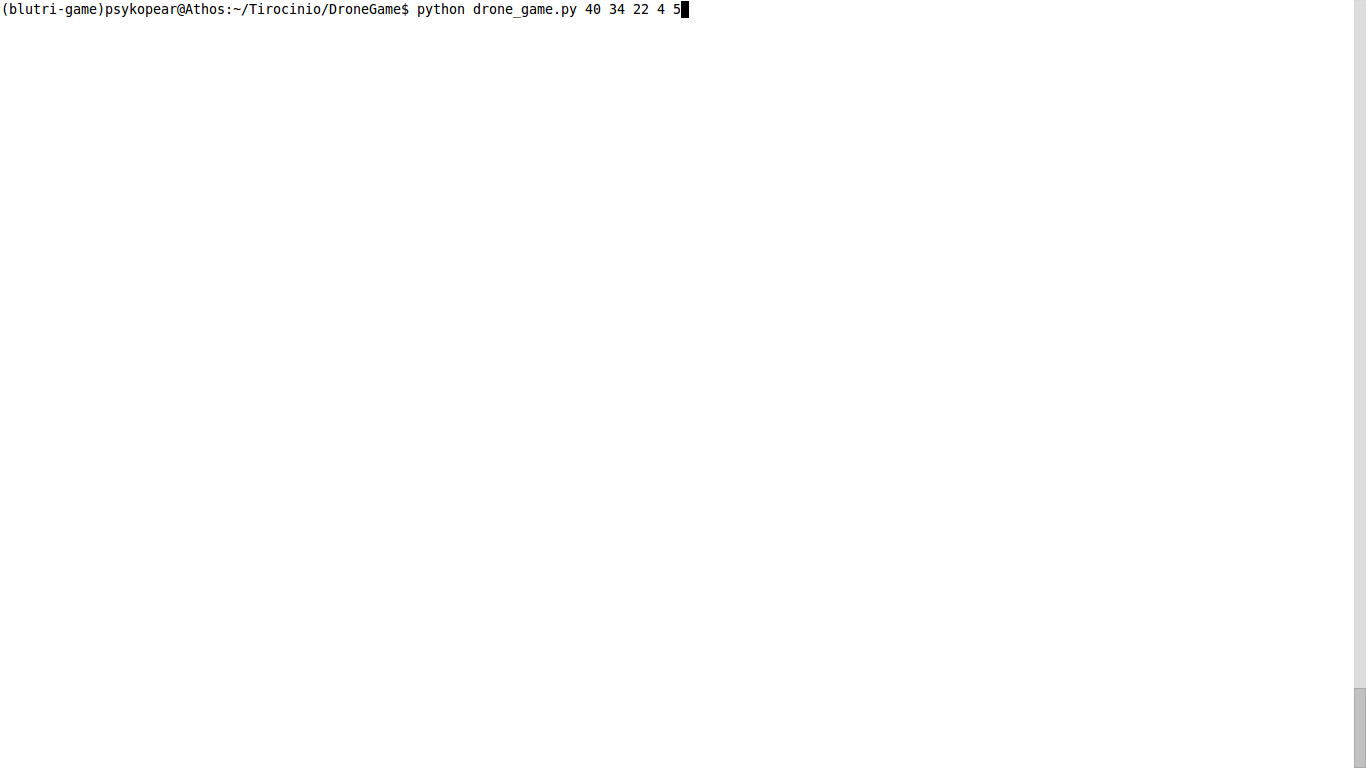
\includegraphics[width=\textwidth]{immagini/Run1.png}
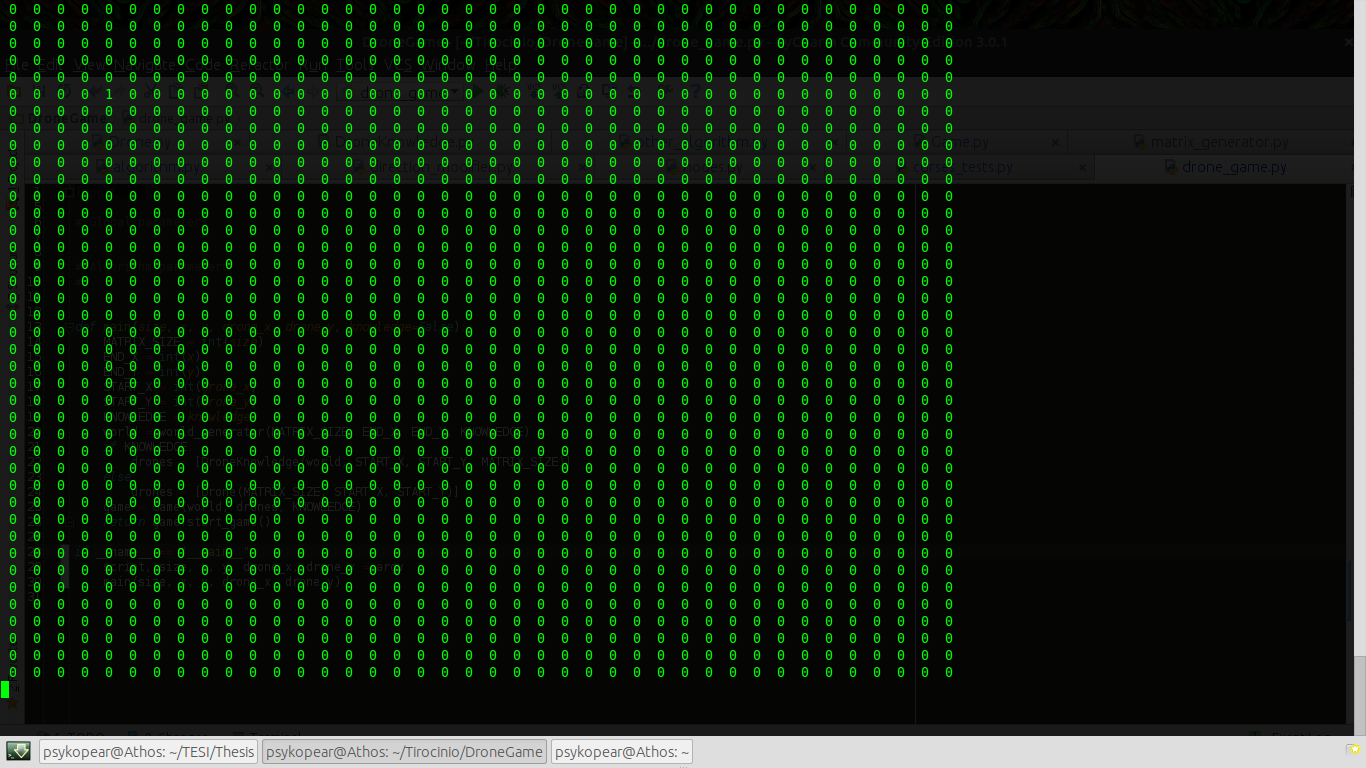
\includegraphics[width=\textwidth]{immagini/Run2.png}
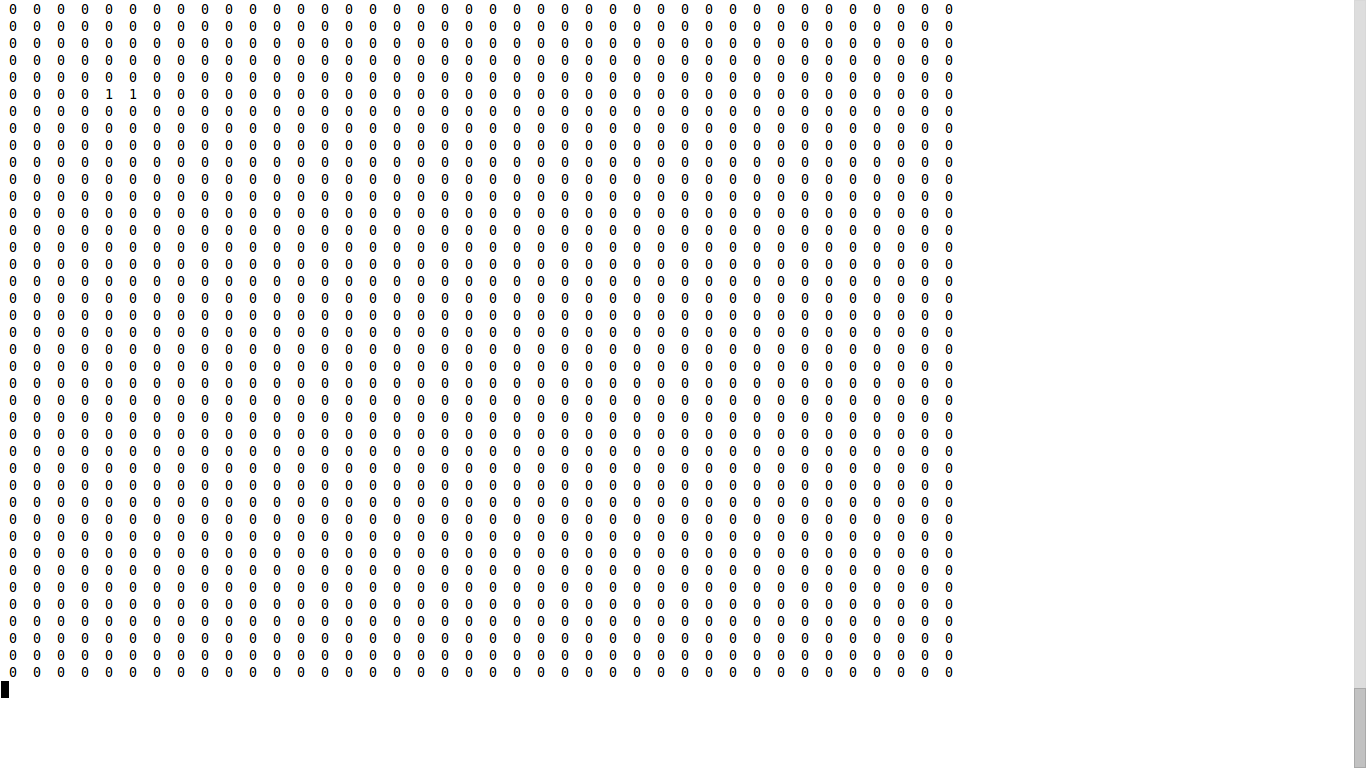
\includegraphics[width=\textwidth]{immagini/Run3.png}
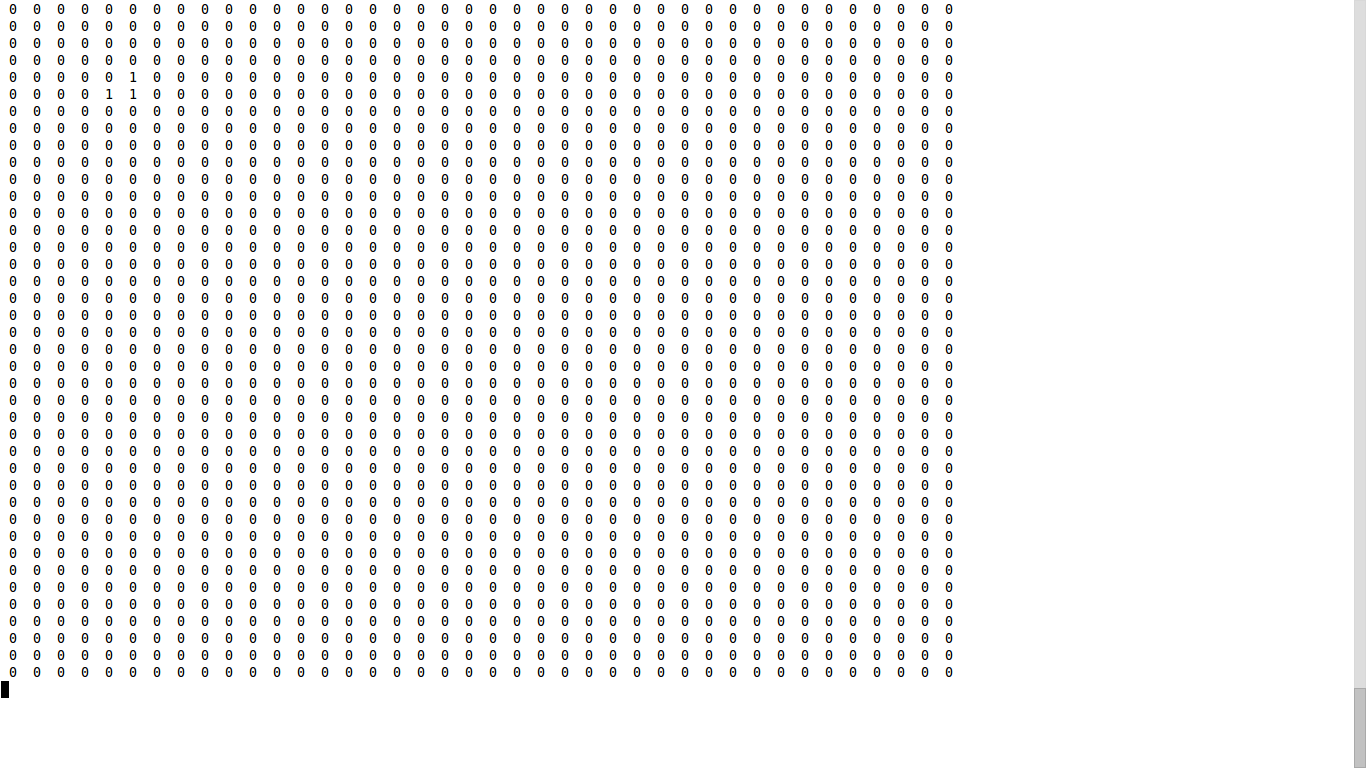
\includegraphics[width=\textwidth]{immagini/Run4.png}
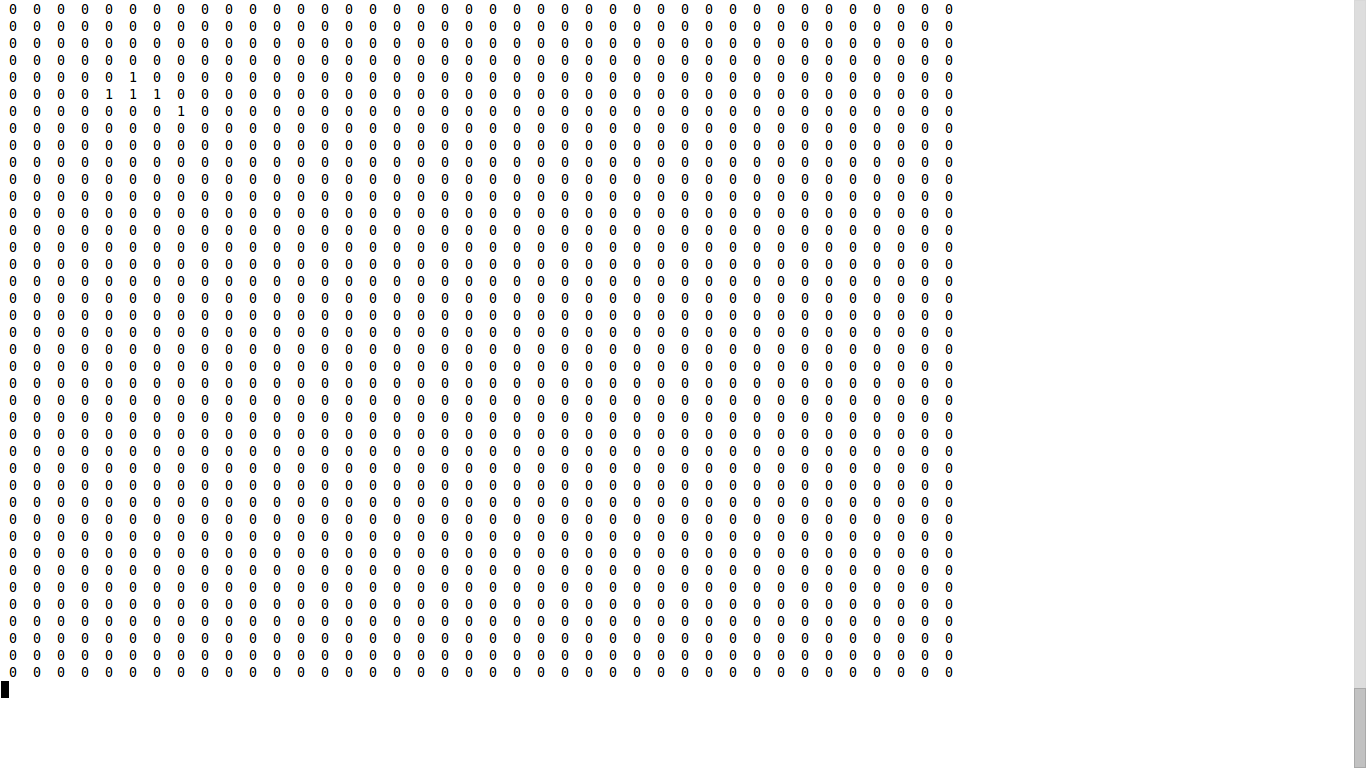
\includegraphics[width=\textwidth]{immagini/Run5.png}
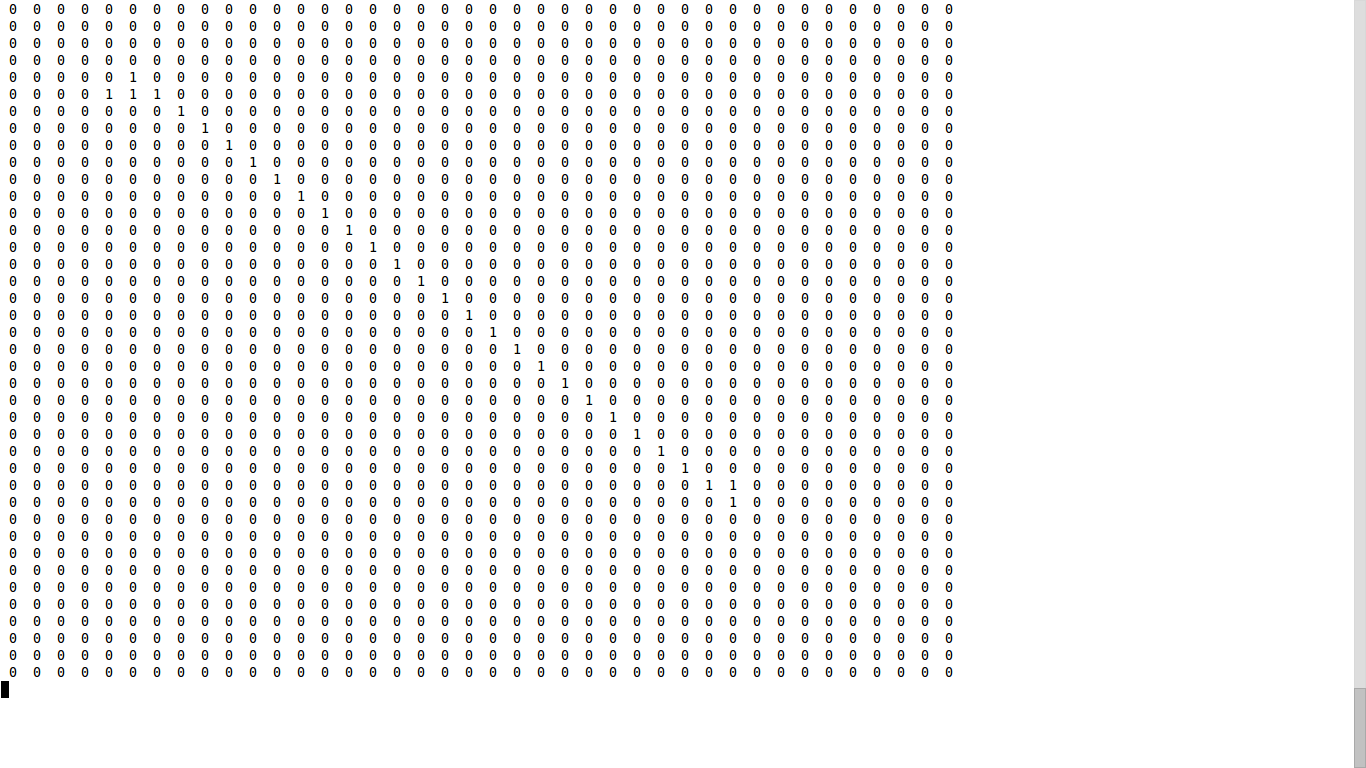
\includegraphics[width=\textwidth]{immagini/Run6.png}
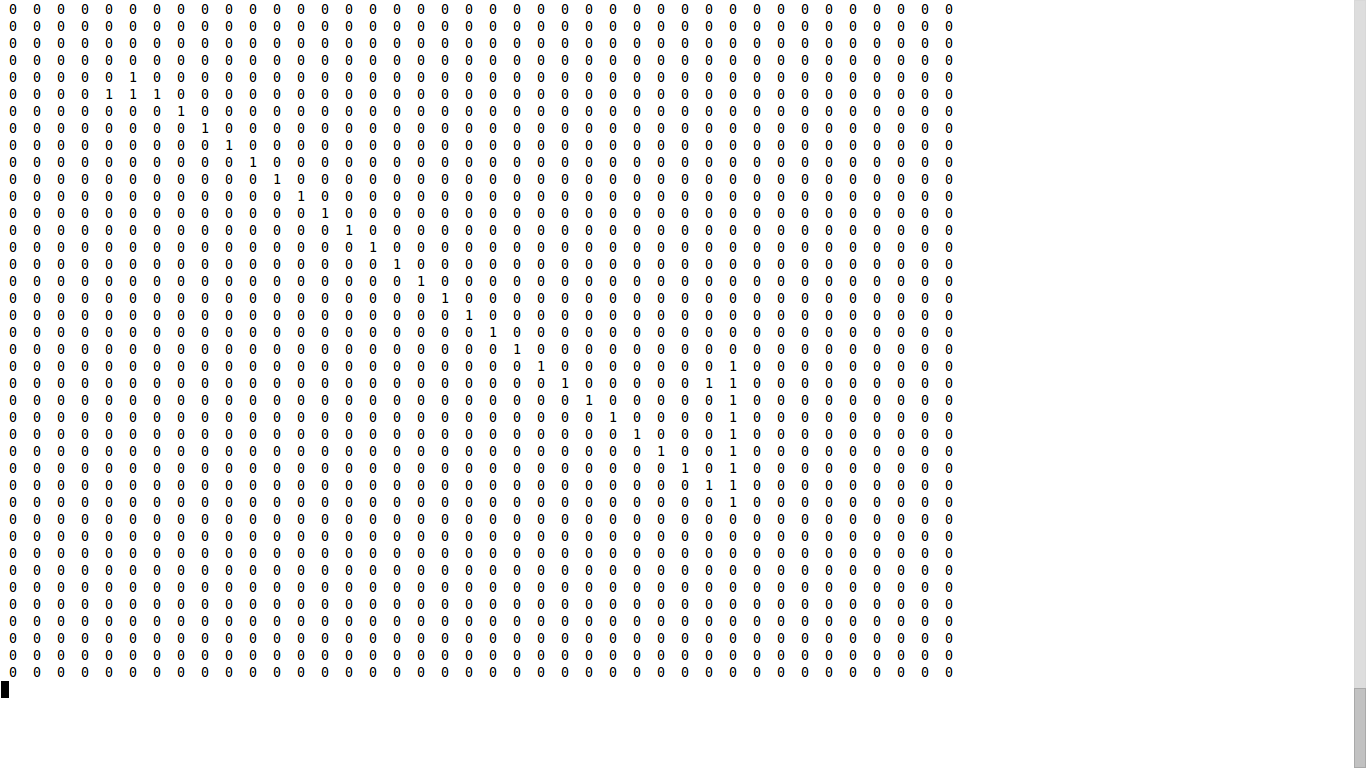
\includegraphics[width=\textwidth]{immagini/Run7.png}
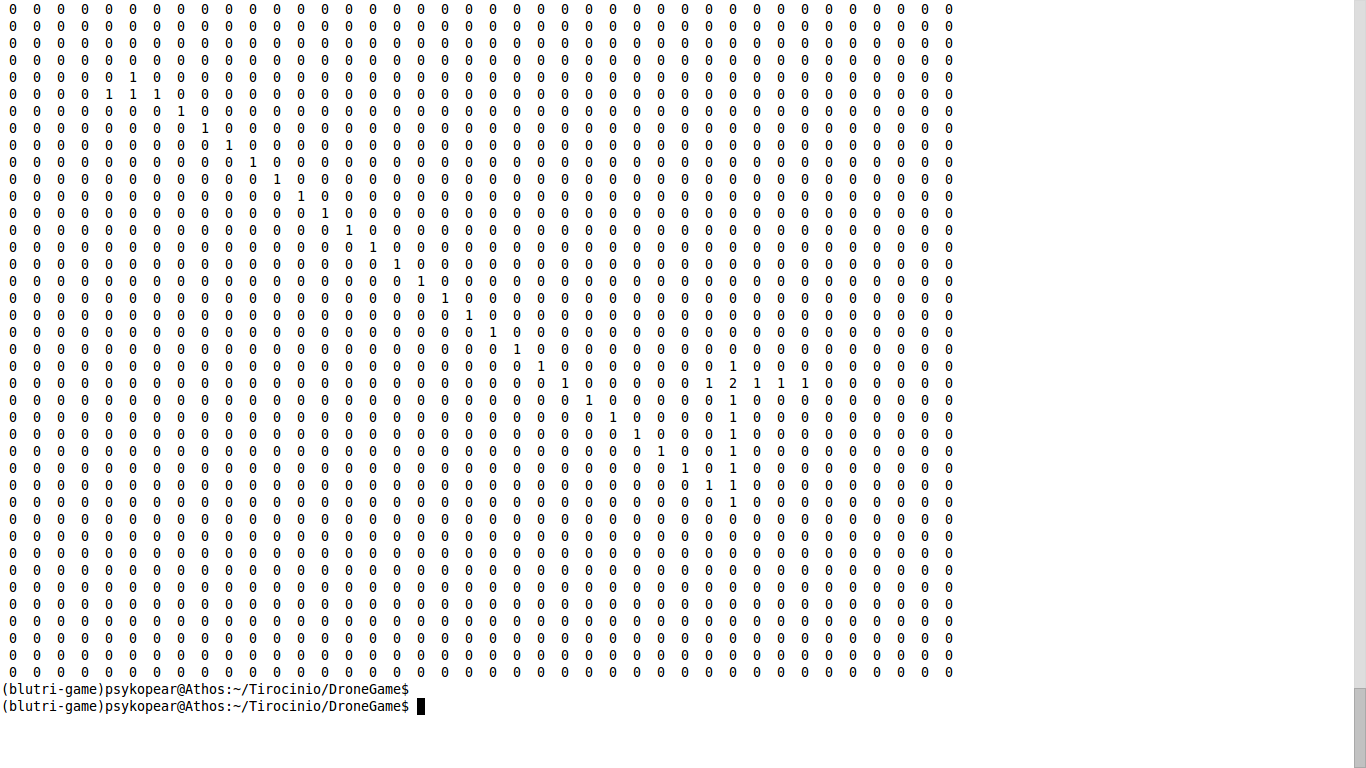
\includegraphics[width=\textwidth]{immagini/Run8.png}
%%%%%%%%%%%%%%%%%%%
%%%%% ESEMPIO:
%\section{index.php}
%\begin{footnotesize}
%\begin{verbatim}
% .... segue file con il codice  ...

\end{document}


